\chapter{FORMALIZAÇÕES COMPLEMENTARES DO PERFIL DE COOPERAÇÃO PREDITIVA}
\label{ap:formalizacao}

O Capítulo~4 define os objetos e indicadores necessários para interpretar os resultados do Capítulo~5. Este apêndice completa essa formalização com o detalhamento de casos, conjuntos auxiliares, a justificativa do armazenamento triangular e exemplos numéricos estendidos, sem os quais algumas afirmações do Capítulo~4 --- em particular sobre empates e sobre a matriz de inversões --- não podem ser verificadas passo a passo.

\section{Resultado par a par observado e os quatro casos de empate}

O resultado par a par observado $U^{(g,f)}_{ij}(n_k)$, definido na Equação~\eqref{eq:observed-outcome}, é recalculado em cada ponto $n_k$ da grade, independentemente do histórico. A relação efetiva de vencedor $W^{(g,f)}_{ij}$, por outro lado, depende de todo o histórico até $n_k$ por meio da regra de propagação da Equação~\eqref{eq:winner-relation}. Isso produz exatamente quatro situações possíveis para um par $(i,j)$ em um ponto $n_k$, $k\geq2$:

\begin{enumerate}
  \item \textbf{Empate inicial não resolvido}: $U_{ij}(n_k)=0$ e $W_{ij}(n_{k-1})=0$ (nenhum vencedor estrito ainda apareceu). Resultado: $W_{ij}(n_k)=0$, permanece indefinido.
  \item \textbf{Primeiro vencedor estrito}: $U_{ij}(n_k)\neq0$ e $W_{ij}(n_{k-1})=0$. Resultado: $W_{ij}(n_k)=U_{ij}(n_k)$, a relação é inicializada.
  \item \textbf{Empate posterior à inicialização}: $U_{ij}(n_k)=0$ e $W_{ij}(n_{k-1})\neq0$. Resultado: $W_{ij}(n_k)=W_{ij}(n_{k-1})$, o vencedor anterior é mantido --- este é o caso que distingue $\Wmat$ do resultado observado $U$, e o único em que a Equação~\eqref{eq:winner-relation} propaga um valor não trivial.
  \item \textbf{Resultado estrito após inicialização}: $U_{ij}(n_k)\neq0$ e $W_{ij}(n_{k-1})\neq0$. Se $U_{ij}(n_k)=W_{ij}(n_{k-1})$, o vencedor é confirmado; se $U_{ij}(n_k)\neq W_{ij}(n_{k-1})$, ocorre uma inversão válida (Seção~\ref{sec:d-reversal-set} abaixo).
\end{enumerate}

Não existe um quinto caso: como $U_{ij}(n_k)\in\{-1,0,+1\}$ e $W_{ij}(n_{k-1})\in\{-1,0,+1\}$, a tabela de $3\times3$ combinações se reduz exatamente aos quatro casos acima porque, sempre que $U_{ij}(n_k)\neq0$, o novo valor de $W_{ij}(n_k)$ é determinado por $U_{ij}(n_k)$ independentemente do sinal específico de $W_{ij}(n_{k-1})$ quando este também é não nulo (casos 2 e 4 coincidem em fórmula, distinguindo-se apenas na interpretação de "inicialização" versus "confirmação/inversão").

\section{Conjunto de eventos de inversão e construção completa de \texorpdfstring{$\Rmat$}{R}}
\label{sec:d-reversal-set}

Para o prefixo terminado em $n_t$, o conjunto de tamanhos amostrais em que o par $(i,j)$ sofreu inversão válida é
\begin{equation}
  \mathcal{E}^{(g,f)}_{ij}(n_t)=
  \left\{
    n_k\leq n_t:
    W^{(g,f)}_{ij}(n_{k-1})\neq0,\;
    W^{(g,f)}_{ij}(n_k)\neq0,\;
    W^{(g,f)}_{ij}(n_k)\neq W^{(g,f)}_{ij}(n_{k-1})
  \right\}.
\end{equation}
A matriz de inversões guarda apenas o mais recente desses eventos, $R^{(g,f)}_{ij}(n_t)=\max\mathcal{E}^{(g,f)}_{ij}(n_t)$ quando $\mathcal{E}^{(g,f)}_{ij}(n_t)\neq\varnothing$, e é indisponível caso contrário (Equação~\eqref{eq:reversal-matrix}). Uma consequência direta é que $\Rmat$ \textbf{descarta} o número total de inversões de um par, sua ordem completa, a duração de cada intervalo entre inversões e a magnitude da perda envolvida em cada uma: dois braços podem compartilhar a última inversão de um par e divergir substancialmente em inversões intermediárias, ou podem discordar sobre a última inversão apesar de exibirem trajetórias de perda praticamente equivalentes (retomado no Capítulo~7, Seção de validade de construto).

\subsection{Justificativa do armazenamento triangular}

A relação efetiva de vencedor satisfaz $W_{ji}(n_k)=-W_{ij}(n_k)$ para todo par com relação definida, por construção da Equação~\eqref{eq:observed-outcome} ($U_{ji}=-U_{ij}$ sempre que $U_{ij}\neq0$) e por indução na regra de propagação (Equação~\eqref{eq:winner-relation}): se $W_{ij}(n_{k-1})=-W_{ji}(n_{k-1})$ vale no passo anterior, então cada um dos quatro casos da seção anterior preserva a antissimetria no passo seguinte, pois $U_{ji}(n_k)=-U_{ij}(n_k)$ e a propagação usa o mesmo ramo da regra para ambas as direções do par. Por isso, armazenar $W_{ij}$ apenas para $i<j$ é suficiente: $W_{ji}$ é recuperável por sinal trocado, e a matriz quadrada exibida nos relatórios (com diagonal vazia e os dois triângulos preenchidos) é uma conveniência de visualização, não uma estrutura de dados adicional. A matriz de inversões $\Rmat$, por não ser antissimétrica --- ela não guarda "quem passou a vencer", apenas "quando a última troca ocorreu" ---, é definida apenas no triângulo superior ($i<j$), e o triângulo inferior é indisponível por definição, não por omissão simétrica.

\subsection{Casos degenerados}

Um par $(i,j)$ pode nunca ter $\Wmat$ definida em todo o prefixo avaliado (empates exatos em todos os pontos da grade); nesse caso, $(i,j)\notin\ReversalSupport_g(n_t)$ para nenhum $n_t$, e o par é excluído tanto do numerador quanto do denominador de $\AR$ (Equação~\eqref{eq:ar}), nunca contado como discordância. Um par pode ter $\Wmat$ definida desde o início e nunca sofrer inversão (um subconjunto domina o outro em toda a grade); esse par também está ausente de $\ReversalSupport_g(n_t)$, indistinguível --- apenas a partir de $\Rmat$ --- do caso anterior. A Seção~\ref{sec:d-reversal-set} já registra essa ambiguidade como uma limitação de construto explícita, retomada no Capítulo~7.

\section{Exemplo numérico estendido}

Considere um par $(S_i,S_j)$ avaliado na grade $n\in\{2,4,8,16,32\}$, com resultados observados $U_{ij}=(0,\,+1,\,0,\,-1,\,0)$. A relação efetiva $\Wmat$ evolui como:

\begin{center}
\begin{tabular}{lccccc}
\toprule
$n_k$ & 2 & 4 & 8 & 16 & 32 \\
\midrule
$U_{ij}(n_k)$ & $0$ & $+1$ & $0$ & $-1$ & $0$ \\
$W_{ij}(n_k)$ & $0$ & $+1$ & $+1$ & $-1$ & $-1$ \\
Caso (Seção D.1) & 1 & 2 & 3 & 4 (inversão) & 3 \\
\bottomrule
\end{tabular}
\end{center}

Em $n=2$, o empate inicial deixa $W_{ij}$ indefinido (caso 1). Em $n=4$, o primeiro vencedor estrito inicializa a relação em $+1$ (caso 2). Em $n=8$, um novo empate exato \emph{mantém} $W_{ij}=+1$ (caso 3) --- é este ponto que distingue $\Wmat$ do resultado observado $U$, que registraria $0$. Em $n=16$, o resultado estrito $-1$ diverge do vencedor efetivo anterior ($+1$): ocorre uma inversão válida, e $16\in\mathcal{E}_{ij}(n_t)$ para todo $n_t\geq16$. Em $n=32$, outro empate mantém o novo vencedor efetivo, $-1$ (caso 3). Para o prefixo $n_t=32$, $R_{ij}(32)=16$ --- o único elemento de $\mathcal{E}_{ij}(32)=\{16\}$ --- e o par pertence a $\ReversalSupport_g(32)$. Se um segundo braço apresentasse sua própria inversão mais recente em $n_k=8$ para o mesmo par, os dois braços concordariam sobre a existência da inversão (contribuindo para $\AR=1$ nesse par) mas divergiriam no regime amostral, com $\left|\log_2 16-\log_2 8\right|=1$ contribuindo para $\DR$.

\section{Matrizes \texorpdfstring{$\Wmat$}{W}/\texorpdfstring{$\Rmat$}{R} completas: SUPPORT2, Random Forest}

A Figura~\ref{fig:wr-matrices-support2-appendix} mostra, com dados reais do cenário SUPPORT2 (execução \textit{full}, $n\leq512$, classificador Random Forest, sete subconjuntos de referência selecionados um por cardinalidade), a matriz de vencedores $\Wmat$ e a matriz de inversões $\Rmat$ lado a lado para os braços \RealToReal{} e \GaussianToReal. Os valores numéricos de $\AR$, $\DR$ e $\SR$ deste braço e classificador são reportados no Capítulo~5 (Seção de resultados do SUPPORT2); esta figura ilustra o objeto matricial do qual esses números derivam.

\begin{figure}[H]
  \centering
  \caption{Matrizes pareadas $\mathbf{W}$ e $\mathbf{R}$ no maior $n$ avaliado do cenário SUPPORT2 (execução \textit{full}, $n\leq512$, cenário 000008), Random Forest}
  \label{fig:wr-matrices-support2-appendix}
  \begin{minipage}[t]{0.48\linewidth}
    \centering
    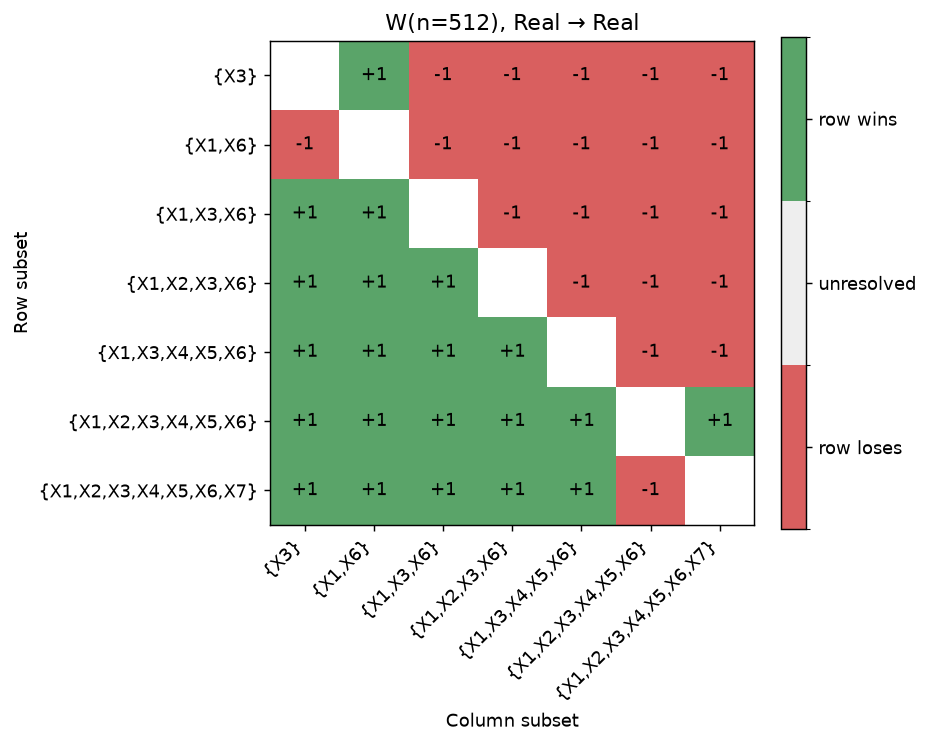
\includegraphics[height=5.4cm,keepaspectratio]{figures/wr_matrices/support2_full/winner_matrix_real_to_real_n512.png}
    \subcaption{$\mathbf{W}(n{=}512)$, \RealToReal}
  \end{minipage}
  \hfill
  \begin{minipage}[t]{0.48\linewidth}
    \centering
    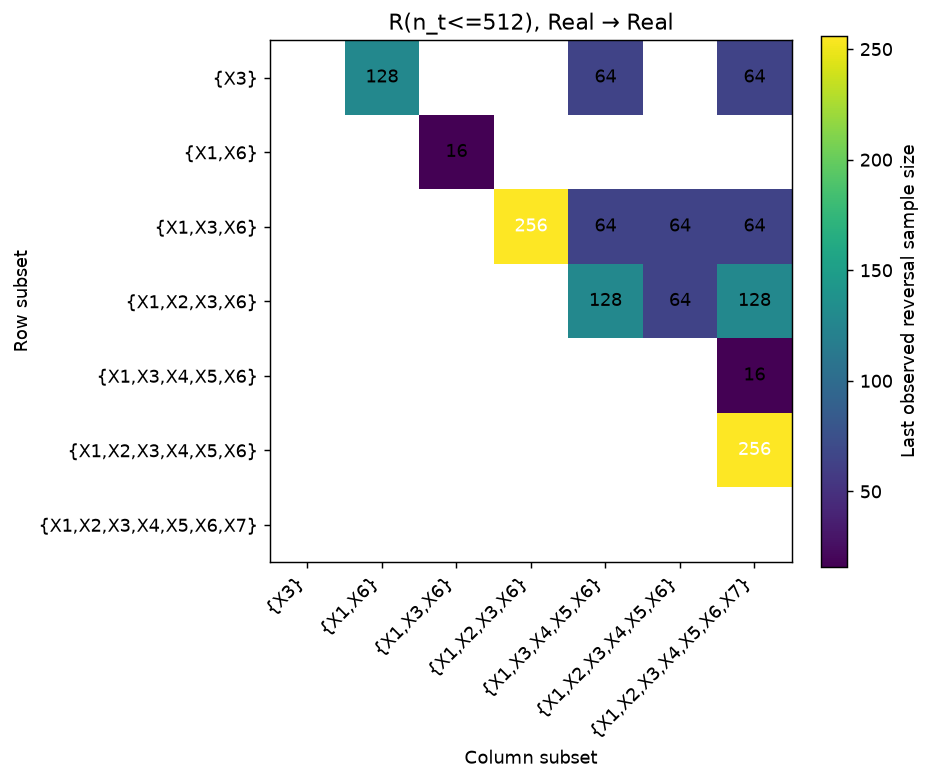
\includegraphics[height=5.4cm,keepaspectratio]{figures/wr_matrices/support2_full/reversal_matrix_real_to_real_n512.png}
    \subcaption{$\mathbf{R}(n_t{\leq}512)$, \RealToReal}
  \end{minipage}

  \vspace{2mm}
  \begin{minipage}[t]{0.48\linewidth}
    \centering
    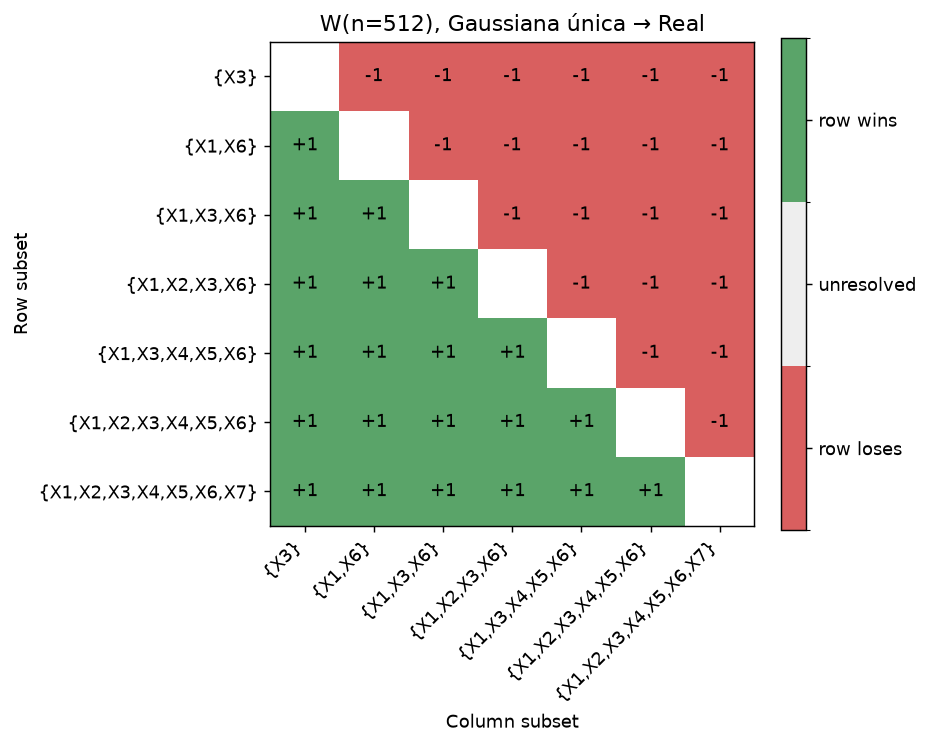
\includegraphics[height=5.4cm,keepaspectratio]{figures/wr_matrices/support2_full/winner_matrix_single_gaussian_to_real_n512.png}
    \subcaption{$\mathbf{W}(n{=}512)$, \GaussianToReal}
  \end{minipage}
  \hfill
  \begin{minipage}[t]{0.48\linewidth}
    \centering
    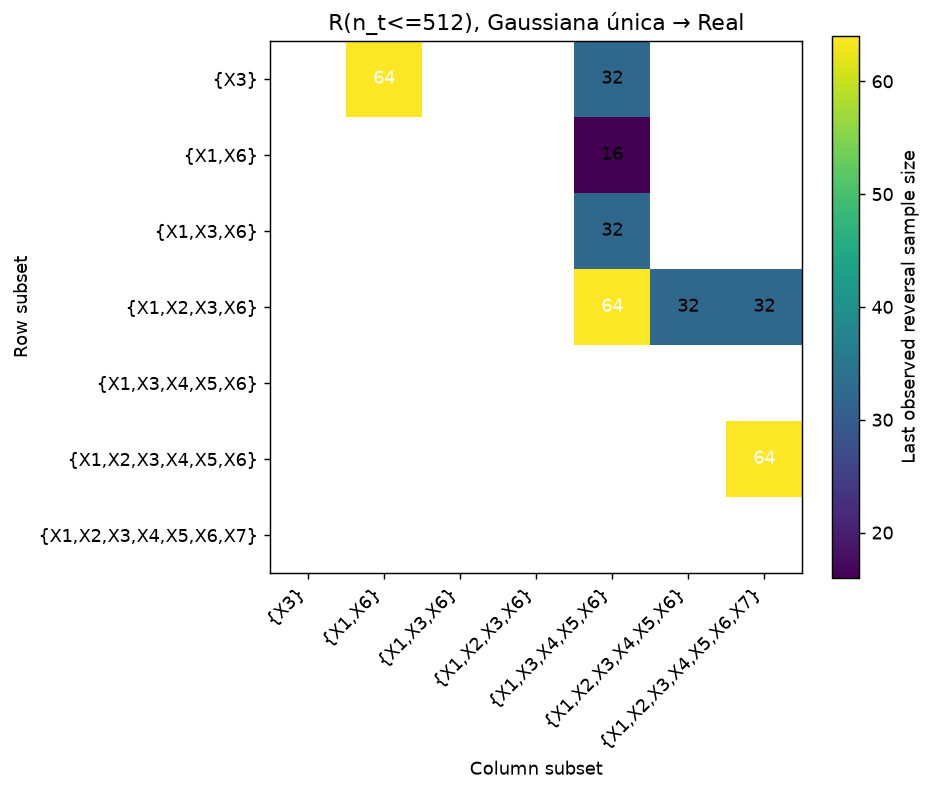
\includegraphics[height=5.4cm,keepaspectratio]{figures/wr_matrices/support2_full/reversal_matrix_single_gaussian_to_real_n512.png}
    \subcaption{$\mathbf{R}(n_t{\leq}512)$, \GaussianToReal}
  \end{minipage}
  \sourcebelow{recomputado diretamente dos resultados brutos por replicação regenerados do cenário SUPPORT2 000008, usando as funções vigentes de \texttt{coinfosim.results.predictive\_profile}; ver Apêndice~B}
  \notailustracao{Sete subconjuntos de referência (um por cardinalidade, selecionados pela menor perda média em $n=512$) entre os 127 do SUPPORT2, para manter a matriz legível; a leitura completa dos 127 subconjuntos permanece disponível no relatório HTML republicado (Apêndice~A)}
\end{figure}

\section{Evolução do resultado par a par observado: exemplo em escala real}

A Figura~\ref{fig:winners-evolucao-appendix} usa o resultado par a par observado do braço \RealToReal{} com SVM linear no cenário Occupancy Detection 000002 --- objeto que corresponde diretamente à comparação $U_{ij}(n)$ da Equação~\eqref{eq:observed-outcome} --- para mostrar como as relações se reorganizam ao longo de toda a grade, de $n=2$ a $n=512$. No início da grade, subconjuntos de baixa cardinalidade vencem muitas comparações porque os modelos maiores sofrem maior variância de estimação; em $n=512$, a organização é mais estável e as combinações informativas passam a vencer uma parcela maior dos pares. O Capítulo~5 (Figura~\ref{fig:occupancy-winner-matrices}) reproduz uma versão compacta dos pontos inicial e final desta mesma sequência.

\begin{figure}[H]
  \centering
  \caption{Evolução do resultado par a par observado no cenário Occupancy Full, braço Real para Real, Linear SVM}
  \label{fig:winners-evolucao-appendix}
  \begin{minipage}[t]{0.31\linewidth}
    \centering
    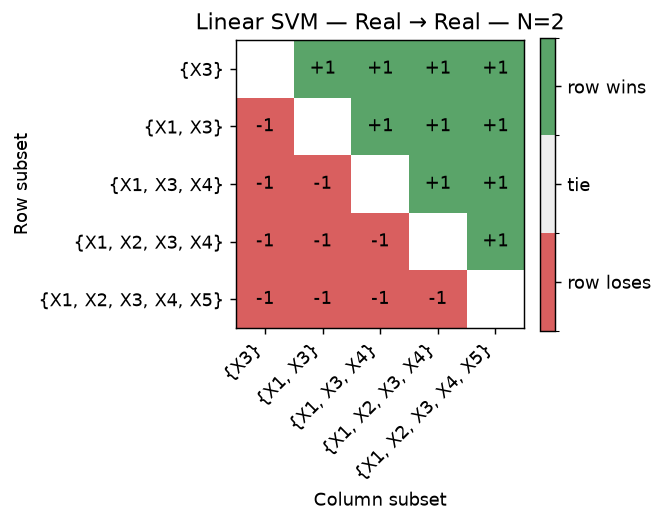
\includegraphics[width=\linewidth]{figures/winners/occupancy/graph_structural_winner_linear_svm_real_to_real_n2_full_000002.png}
    \subcaption{Início: $n=2$}
  \end{minipage}
  \hfill
  \begin{minipage}[t]{0.31\linewidth}
    \centering
    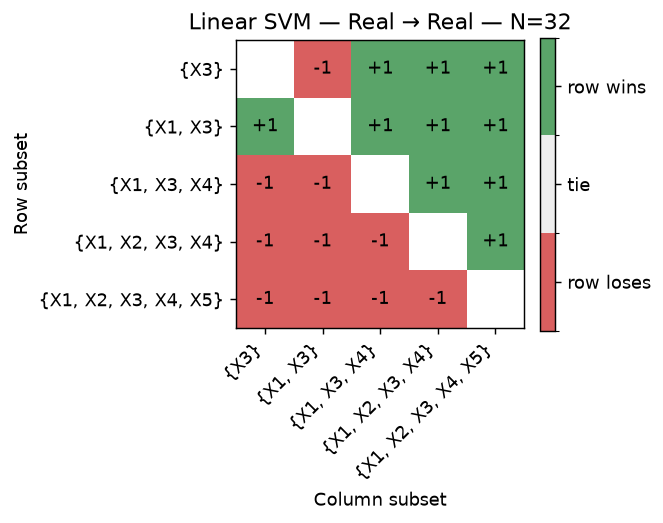
\includegraphics[width=\linewidth]{figures/winners/occupancy/graph_structural_winner_linear_svm_real_to_real_n32_full_000002.png}
    \subcaption{Prefixo intermediário: $n=32$}
  \end{minipage}
  \hfill
  \begin{minipage}[t]{0.31\linewidth}
    \centering
    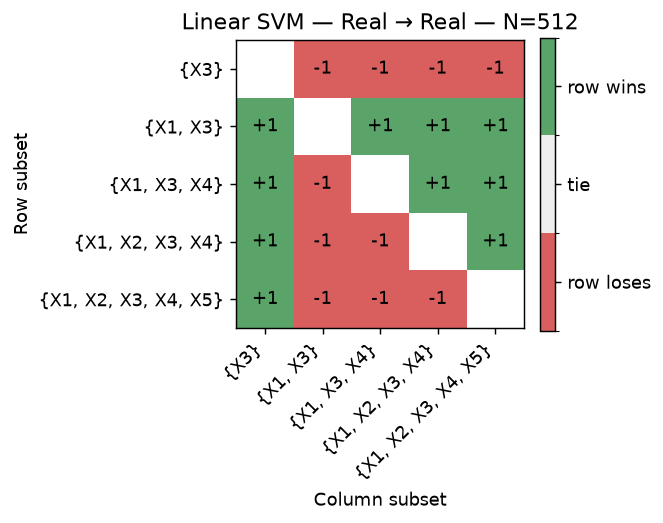
\includegraphics[width=\linewidth]{figures/winners/occupancy/graph_structural_winner_linear_svm_real_to_real_n512_full_000002.png}
    \subcaption{Fim: $n=512$}
  \end{minipage}
  \sourcebelow{relatório publicado do cenário Occupancy Detection 000002 do \CoInfoSim}
  \notailustracao{A visualização é quadrada e redundante: a diagonal não se aplica e um triângulo determina o outro fora dos casos indefinidos. Cada célula indica se o subconjunto da linha vence ($+1$), perde ($-1$) ou está indefinido ($0$) contra o subconjunto da coluna. Os painéis exibem os melhores subconjuntos de cada cardinalidade; em $n=2$ o subconjunto singular $\{X_3\}$ vence todas as comparações exibidas, em $n=32$ o par $\{X_1,X_3\}$ já o supera e em $n=512$ as combinações maiores vencem o singular}
\end{figure}
